\chapter{Proverb 13}

\begin{figure}
  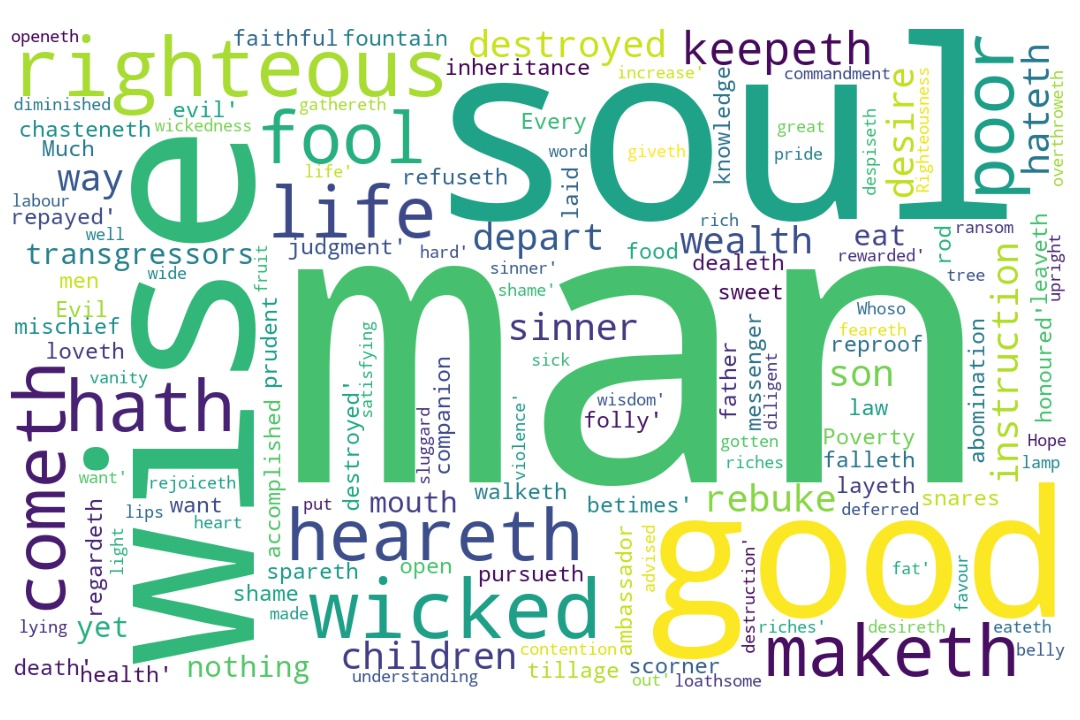
\includegraphics[width=\linewidth]{20OT-Proverbs/Proverb13-WordCloud.jpg}
  \caption{Proverb 13 Word Cloud}
  \label{fig:Proverb 13 Word Cloud}
\end{figure}

\marginpar{\scriptsize \centering \fcolorbox{bone}{lime}{\textbf{A WISE MAN}}\\ (Proverbs 13:1-25) \begin{compactenum}[I.][8]
    \item \textbf{Hears Instruction} \index[scripture]{Proverbs!Pro 13:01}(Pro 13:1)
    \item \textbf{Holds His Tongue} \index[scripture]{Proverbs!Pro 13:03}(Pro 13:3)
    \item \textbf{Hates Lying} \index[scripture]{Proverbs!Pro 13:05}(Pro 13:5)
    \item Is \textbf{Held up by Righteousness} \index[scripture]{Proverbs!Pro 13:06}(Pro 13:6)
    \item \textbf{Has True Wealth} \index[scripture]{Proverbs!Pro 13:07}(Pro 13:7)
    \item \textbf{Hearkens to God's Word} \index[scripture]{Proverbs!Pro 13:13}(Pro 13:13)
    \item \textbf{Hangs out with other wise Men} \index[scripture]{Proverbs!Pro 13:20}(Pro 13:20)
\end{compactenum}}

\marginpar{\scriptsize \centering \fcolorbox{bone}{yellow}{\textbf{A WISE SON}}\\ (Proverbs 13:1-25) \begin{compactenum}[I.][8]
    \item \textbf{Listens} to Instruction \index[scripture]{Proverbs!Pro 13:01}(Pro 13:1)
    \item \textbf{Learns}  \index[scripture]{Proverbs!Pro 13:01}(Pro 13:1)
    \item \textbf{Locks} his Lips \index[scripture]{Proverbs!Pro 13:03}(Pro 13:3)
    \item \textbf{Labours}  \index[scripture]{Proverbs!Pro 13:11}(Pro 13:11)
    \item \textbf{Likes} Reproof \index[scripture]{Proverbs!Pro 13:18}(Pro 13:18)
    \item \textbf{Leaves} an Inheritance \index[scripture]{Proverbs!Pro 13:22}(Pro 13:22)
    \item \textbf{Loves} Enough to Correct \index[scripture]{Proverbs!Pro 13:24}(Pro 13:24)
\end{compactenum}}

\footnote{\textcolor[cmyk]{0.99998,1,0,0}{\hyperlink{TOC}{Return to end of Table of Contents.}}}\footnote{\href{https://www.audioverse.org/english/audiobibles/books/ENGKJV/O/Prov/1}{\textcolor[cmyk]{0.99998,1,0,0}{Proverbs Audio}}}\textcolor[cmyk]{0.99998,1,0,0}{A wise son \fcolorbox{bone}{lime}{\emph{heareth} his father's instruction}: but a scorner heareth not rebuke.}\footnote{\textbf{Isaiah 29:20} - For the terrible one is brought to nought, and the scorner is consumed, and all that watch for iniquity are cut off:}
[2] \textcolor[cmyk]{0.99998,1,0,0}{A man \fcolorbox{bone}{bone}{shall} eat good by the fruit of \emph{his} mouth: but the soul of the \fcolorbox{bone}{MYGOLD}{transgressors} \emph{\fcolorbox{bone}{bone}{shall}} \emph{eat} violence.}
[3] \textcolor[cmyk]{0.99998,1,0,0}{He that \fcolorbox{bone}{lime}{keepeth his mouth} keepeth his life: \emph{but} he that openeth wide his lips \fcolorbox{bone}{bone}{shall} have destruction.}
[4] \textcolor[cmyk]{0.99998,1,0,0}{The soul of the sluggard desireth, and \emph{hath} nothing: but the soul of the diligent \fcolorbox{bone}{bone}{shall} be made fat.}
[5] \textcolor[cmyk]{0.99998,1,0,0}{A righteous \emph{man} \fcolorbox{bone}{lime}{hateth lying}: but a wicked \emph{man} is loathsome, and cometh to shame.}
[6] \textcolor[cmyk]{0.99998,1,0,0}{\fcolorbox{bone}{MYGOLD}{Righteousness} keepeth \emph{him} \emph{that} \emph{is} upright in the way: but wickedness overthroweth the sinner.}
[7] \textcolor[cmyk]{0.99998,1,0,0}{There is that maketh himself rich, yet \emph{hath} nothing: \emph{there} \emph{is} that maketh himself poor, \fcolorbox{bone}{lime}{yet \emph{hath} great riches}.}
[8] \textcolor[cmyk]{0.99998,1,0,0}{The ransom of a man's life \emph{are} his riches: but the poor heareth not rebuke.}
[9] \textcolor[cmyk]{0.99998,1,0,0}{The light of the righteous rejoiceth: but the lamp of the wicked \fcolorbox{bone}{bone}{shall} be put out.}
[10] \textcolor[cmyk]{0.99998,1,0,0}{Only by pride cometh contention: but with the well advised \emph{is} wisdom.}
[11] \textcolor[cmyk]{0.99998,1,0,0}{Wealth \emph{gotten} by vanity \fcolorbox{bone}{bone}{shall} be diminished: but he that gathereth by labour \fcolorbox{bone}{bone}{shall} increase.}
[12] \textcolor[cmyk]{0.99998,1,0,0}{Hope deferred maketh the heart sick: but \emph{when} the desire cometh, \emph{it} \emph{is} a tree of life.}
[13] \textcolor[cmyk]{0.99998,1,0,0}{Whoso despiseth the word \fcolorbox{bone}{bone}{shall} be destroyed: but he that \fcolorbox{bone}{lime}{feareth the commandment} \fcolorbox{bone}{bone}{shall} be rewarded.}
[14] \textcolor[cmyk]{0.99998,1,0,0}{The law of the wise \emph{is} a fountain of life, to depart from the snares of death.}
[15] \textcolor[cmyk]{0.99998,1,0,0}{Good \fcolorbox{bone}{MYGOLD}{understanding} giveth favour: but the way of \fcolorbox{bone}{MYGOLD}{transgressors} \emph{is} hard.}
[16] \textcolor[cmyk]{0.99998,1,0,0}{Every prudent \emph{man} dealeth with knowledge: but a fool layeth open \emph{his} folly.}
[17] \textcolor[cmyk]{0.99998,1,0,0}{A wicked messenger falleth into mischief: but a faithful ambassador \emph{is} health.}
[18] \textcolor[cmyk]{0.99998,1,0,0}{Poverty and shame \emph{\fcolorbox{bone}{bone}{shall}} \emph{be} \emph{to} him that refuseth instruction: but he that regardeth reproof \fcolorbox{bone}{bone}{shall} be honoured.}
[19] \textcolor[cmyk]{0.99998,1,0,0}{The desire accomplished is sweet to the soul: but \emph{it} \emph{is} abomination to fools to depart from evil.}
[20] \textcolor[cmyk]{0.99998,1,0,0}{He that \fcolorbox{bone}{lime}{walketh with wise \emph{men}} \fcolorbox{bone}{bone}{shall} be wise: but a companion of fools \fcolorbox{bone}{bone}{shall} be destroyed.}\footnote{\textbf{2 Kings 9:11} - Then Jehu came forth to the servants of his lord: and one said unto him, Is all well? wherefore came this mad fellow to thee? And he said unto them, Ye know the man, and his communication.}\footnote{\textbf{1 Corinthians 15:33} - Be not deceived: evil communications corrupt good manners.}
[21] \textcolor[cmyk]{0.99998,1,0,0}{Evil pursueth sinners: but to the righteous good \fcolorbox{bone}{bone}{shall} be repayed.}
[22] \textcolor[cmyk]{0.99998,1,0,0}{A good \emph{man} leaveth an inheritance to his children's children: and the wealth of the sinner \emph{is} laid up for the just.}
[23] \textcolor[cmyk]{0.99998,1,0,0}{Much food \emph{is} \emph{in} the tillage of the poor: but there is \emph{that} \emph{is} destroyed for want of judgment.}
[24] \textcolor[cmyk]{0.99998,1,0,0}{He that spareth his rod hateth his son: but he that loveth him chasteneth him betimes.}
[25] \textcolor[cmyk]{0.99998,1,0,0}{The righteous eateth to the satisfying of his soul: but the belly of the wicked \fcolorbox{bone}{bone}{shall} want.}


% ransom , rebuke, refuseth, regardeth, rejoiceth, repayed, reproof, rewarded, rich, riches, righteous, rod
